\chapter{Dataset PTN}
\label{cap1}

\section{Introduzione al dataset}
L'analisi presentata si basa sui dati resi disponibili dal \textbf{Portale Open Data del Comune di Milano} che fornisce in formato aperto numerose informazioni relative alla città, incluse quelle sul \textit{trasporto pubblico locale} \cite{ComuneMilanoOpenData}. In particolare, i dati sul trasporto pubblico sono forniti dall'\textbf{Agenzia Mobilità Ambiente Territorio} \cite{Amat}, società che, tra le altre cose, si occupa di raccogliere, gestire e diffondere i \textit{dati sulla mobilità urbana}.

Tale società fornisce i dati in formato GTFS \cite{GTFS}, uno standard che, attraverso un insieme di file, permette di rappresentare digitalmente un'intera rete di trasporto, integrando anche dati geografici e temporali. Fornisce inoltre gli stessi dati anche in un formato \textit{proprietario}, strutturato in file csv in lingua italiana che perdono parte delle informazioni del GTFS, ma che sono comunque completi rispetto alla struttura e ai collegamenti della rete.

Per questo motivo e considerando le finalità dell'analisi, si è scelto di utilizzare il \textit{formato proprietario}.

\section{Esplorazione dei dataset}
Il dataset si compone di tre dataset che sono reperibili indipendentemente gli uni dagli altri:
\begin{itemize}
    \item \textbf{Fermate linee metropolitane} dataset contenente le informazioni sulle fermate di tutte le linee metropolitane \cite{FermateLineeMetropolitane};
    \item \textbf{Percorsi linee metropolitane} dataset contenente le informazioni su tutti i percorsi che compongono le linee, che non sono unicamente quelli tra due fermate di capolinea, ma anche quelli percorribili tra tutte le fermate che consentono l'inversione del verso di percorrenza \cite{PercorsiLineeMetropolitane};
    \item \textbf{Composizione percorsi linee metropolitane} dataset contenente le informazioni sui collegamenti dei percorsi, ovvero quali fermate li compongono e come sono tra loro collegate \cite{ComposizionePercorsiLineeMetropolitane}.
\end{itemize}

\subsection{Composizione dei dataset}
Complessivamente, si tratta di $130$ fermate metropolitane che servono $43$ percorsi metropolitani per un totale di $838$ collegamenti. Gli attributi di ogni dataset sono descritti nelle tabelle \ref{tab:Attributi del dataset dei Percorsi}, \ref{tab:Attributi del dataset delle Fermate}, \ref{tab:Attributi del dataset della Composizione dei Percorsi}.

\begin{table}[!ht]
\centering
\begin{tabular}{lll}
\hline
\textbf{Attributo} & \textbf{Tipo} & \textbf{Descrizione} \\
\hline
\texttt{\_id} & int64 & ID numerico univoco del percorso \\
\texttt{linea} & int64 & Numero di linea \\
\texttt{mezzo} & object & Mezzo (METRO) \\
\texttt{percorso} & int64 & Codice numerico univoco del percorso \\
\texttt{nome} & object & Nome del percorso \\
\texttt{lung\_km} & float64 & Lunghezza in Km \\
\texttt{num\_ferm} & int64 & Numero di fermate \\
\texttt{LONG\_X\_4326\_CENTROID} & float64 & Geometria del percorso - longitudine \\
\texttt{LAT\_Y\_4326\_CENTROID} & float64 & Geoemtria del percorso - latitudine \\
\texttt{Location} & object & Geometria del percorso  \\
\hline
\end{tabular}
\caption{Attributi del dataset dei Percorsi}
\label{tab:Attributi del dataset dei Percorsi}
\end{table}

\begin{table}[ht!]
\centering
\begin{tabular}{lll}
\hline
\textbf{Attributo} & \textbf{Tipo} & \textbf{Descrizione} \\
\hline
\texttt{\_id} & int64 & ID numerico univoco della fermata \\
\texttt{id\_amat} & int64 & ID Amat della fermata \\
\texttt{nome} & object & Nome della fermata \\
\texttt{linee} & object & Codici delle linee che transitano per la fermata \\
\texttt{LONG\_X\_4326} & float64 & Longitudine della posizione della fermata \\
\texttt{LAT\_Y\_4326} & float64 & Latitudine della posizione della fermata \\
\texttt{Location} & object & Geometria del percorso  \\
\hline
\end{tabular}
\caption{Attributi del dataset delle Fermate}
\label{tab:Attributi del dataset delle Fermate}
\end{table}

\begin{table}[ht!]
\centering
\begin{tabular}{lll}
\hline
\textbf{Attributo} & \textbf{Tipo} & \textbf{Descrizione} \\
\hline
\texttt{\_id} & int64 & ID numerico del componente del percorso \\
\texttt{percorso} & int64 & Codice numerico del percorso \\
\texttt{num} & int64 & Numero di sequenza della fermata lungo il percorso \\
\texttt{id\_ferm} & int64 & ID numerico della fermata coinvolta \\
\hline
\end{tabular}
\caption{Attributi del dataset della Composizione dei Percorsi}
\label{tab:Attributi del dataset della Composizione dei Percorsi}
\end{table}

\subsection{Qualità dei dataset}
I dataset sono aggiornati rispetto alla formazione più recente della rete metropolitana, presentando come data di ultima modifica il \textit{16 ottobre 2024} \cite{FermateLineeMetropolitane}\cite{PercorsiLineeMetropolitane}\cite{ComposizionePercorsiLineeMetropolitane}. Non presentano incogruenze o rumori di alcun tipo, così come non presentano valori mancanti.

\section{Analisi dei dataset}
I dataset si riconducono alla struttura dei file GTFS, il cui scopo principale è descrivere una rete di trasporto e non analizzarla, pertanto si compone di molti attributi che non hanno un vero e proprio valore da punto di vista analitico, come informazioni sulle posizioni geografiche e id univoci di riferimento.

D'altra parte, i tre dataset in studio hanno comunque alcuni attributi che possono essere utili per fornire una prima analisi della rete metropolitana, che potrà poi essere approfondita nello studio del grafo derivante.

\subsection{Analisi del dataset delle Fermate}
\label{subsec: analisi del dataset dellef ermate}
In totale sono presenti $130$ fermate ognuna con un id \textbf{univoco}, anche se alcune identificate con id diversi sono, in realtà, la stessa fermata. Può sembrare una considerazione banale, ma la diversa \textbf{nomenclatura} di una stessa stazione dovrà essere gestita in fase di costruzione del grafo di rappresentazione della rete per evitare errori.

Le linee alle quali appartengono le fermate sono $5$, corrispondenti alle cinque linee che compongono la rete: \textit{M1}, \textit{M2}, \textit{M3}, \textit{M4} e \textit{M5}. La linea più frequenze è la \textbf{linea 1} presente $37$ volte,  il che suggerisce sia la linea con più fermate delle cinque.

\subsection{Analisi del dataset dei Percorsi}
I percorsi disponibili sono $43$, questo dato suggerisce che i percorsi identificati in questo dataset non siano unicamente quelli tra stazioni capolinea, ma anche quelli tra stazioni che consentono ai treni di effettuare un'\textbf{inversione di marcia} grazie alla presenza di specifici binari di manovra o raccordi.

\vspace{1.5em}
\begin{table}[h!]
\centering
\begin{tabular}{lll}
\hline
\textbf{Linea} & \textbf{Percorsi} \\
\hline
M1 & 27 \\
M2 & 10 \\
M3 & 2 \\
M4 & 2 \\
M5 & 2 \\
\hline
\end{tabular}
\caption{Numero di percorsi per ogni linea}
\label{tab:Numero di percorsi per ogni linea}
\end{table}
\vspace{1.5em}

Dal conteggio dei percorsi in tabella \ref{tab:Numero di percorsi per ogni linea} si può anche dedurre che le uniche linee che consentono l'operazione sopra descritta sono la \textit{linea 1} e la \textit{linea 2}.

Ogni percorso è composto da una \textbf{media} di $20$ fermate, con una \textbf{lunghezza} media di $19$ chilometri.

\subsection{Analisi del dataset della Composizione dei Percorsi}
Questo dataset può essere visto come una \textit{descrizione delle relazioni} tra i due dataset precedenti, ovvero descrive quali fermate e in che ordine compongono i percorsi, pertanto non espone alcun interesse dal punto di vista analitico.

\section{Preprocessamento dei dataset}

\subsection{Data cleaning}
I dati sono ben rappresentati nei dataset e non presentano valori nulli, come evidenziato dall'inizio del capitolo \ref{cap1}. non è stato quindi necessario svolgere alcuna operazione in questa fase.

\subsection{Data transformation}
I dati sono tutti rappresentati nei formati corretti e non hanno bisogno di operazioni di normalizzazione o aggregazione. L'unico attributo che ha richiesto un processamento è l'attributo \texttt{linee} che è stato convertito in una \textit{lista di interi}, originalmente era infatti rappresentato come una stringa contenente i numeri di linee intercalate da virgole.

\subsection{Feature selection e Data Integration}

Rispetto ai dataset iniziali, gli attributi mantenuti sono quelli visibili in figura \ref{fig:data integration}.

\vspace{1em}
\begin{figure}[h!]
    \centering
    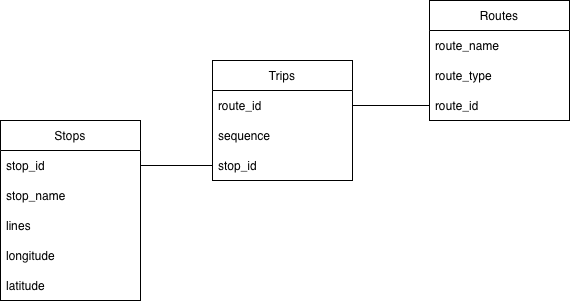
\includegraphics[width=0.7\linewidth]{Immagini/Capitoli/cap1/data_integration.png}
    \caption{Relazioni tra i dataset ridotti}
    \label{fig:data integration}
\end{figure}
\vspace{1em}

La figura \ref{fig:data integration} presenta anche le relazioni esistenti tra i dataset. Ai fini della costruzione del grafo sono stati comunque mantenuti separati, poiché questa scelta agevolava le iterazioni sui dati necessarie alla costruzione del grafo.